\enteteThematiqueObligatoire{}
\enteteCorrection{}

\subsection*{Système d'asservissement de position d'un faisceau LASER}

Dans ce TD, on se propose d'étudier un \textbf{système réel}, son \textbf{modèle} et son \textbf{asservissement corrigé}.

\begin{center}
	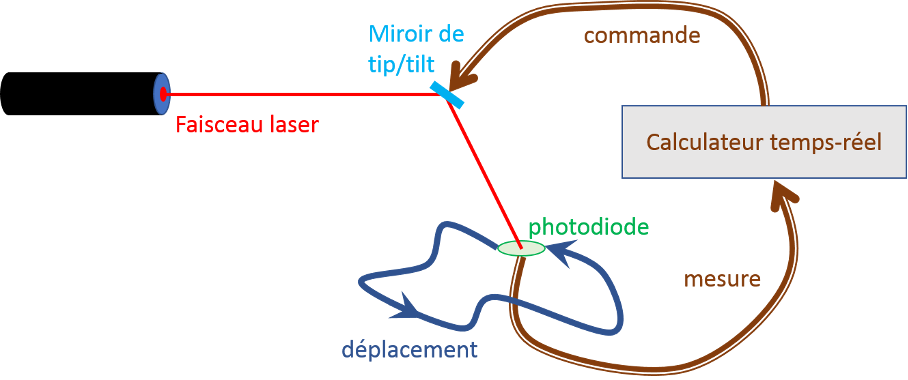
\includegraphics[width=12cm]{images/TD/systBoucle.png}
\end{center}


Le système à étudier permet de positionner un \textbf{pointeur LASER} à l'aide de deux moteurs galvanométriques (eux-mêmes asservis en position) selon deux directions (X et Y). L'information est récupérée par une photodiode 4 quadrants.

\begin{center}
	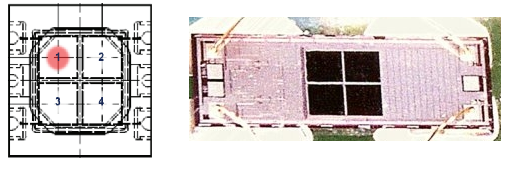
\includegraphics[width=8cm]{images/TD/4q_photodiode.png}
\end{center}

Seule la voie X sera étudiée ici, les deux directions étant équivalentes.

Les moteurs galvanométriques sont pilotés à l'aide d'une tension et asservis en angle. Pour une tension donnée le "servomoteur" se positionnera à un angle particulier.

Le capteur de position (la photodiode 4 quadrants) renvoie une tension en lien avec la position du faisceau LASER.

\subsection*{Application à l'optique adaptative}

Dans de nombreuses applications, on utilise des lasers dont le faisceau doit être pointé sur une cible avec une grande précision. Par exemple lorsque l'on crée des étoiles artificielles pour l'observation astronomique par optique adaptative, les étoiles artificielles doivent être créées à une certaine position angulaire et à une certaine altitude. La présence de l'atmosphère fait dévier le faisceau, et ces déviations peuvent être compensées par des petits miroirs plans dits de basculement (ou de tip/tilt) grâce à un asservissement utilisant la mesure des écarts à la position voulue.

\textit{Voir TP de 3A en optique adaptative.}


%%%%%%%%%%%%%%%%%%%%%%%%%%%%%%%%%%%%%%%%%%%%%%%%%%%%%%%%%%%%%%%%%%
\encadreTDExo{1 - Modèle du système}{
\begin{itemize}[label=$\triangleright$,leftmargin=*]
	\item Caractérisation en fréquence d'un système et identification de paramètres
	\item Lien avec la réponse à un échelon
\end{itemize}
}

Il a été montré expérimentalement que le système complet (servomoteur) pouvait être modélisé par la relation suivante (dans sa zone de fonctionnement linéaire) :

$$T(p) = \frac{G_0}{1 + \frac{2 \cdot m \cdot p}{w_c} + \frac{p^2}{w_c^2}}$$

Le capteur peut être modélisé par un simple gain qu'on notera $K_{capt} = 10$.

\begin{enumerate}
	\item Tracez le schéma bloc du système.
	\answer{
		\begin{center}
			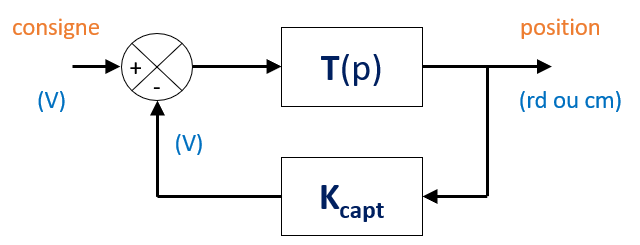
\includegraphics[width=10cm]{images/TD/syst_boucle_schema.png}
		\end{center}
	}
	
	\item De quel type est ce système ? Quelles sont les grandeurs d'entrée et de sortie des différents blocs ?
	\answer{
		Ce système est du second ordre en boucle ouverte.
		
		L'entrée est une tension de consigne. Le système "servomoteur" $T(p)$ transforme cette tension en une position en X (ou Y). Le capteur permet de transformer une position en une tension.	
	}
	
	\medskip
	
	On donne le relevé expérimental de la réponse à un échelon de ce système :
	
\begin{center}
	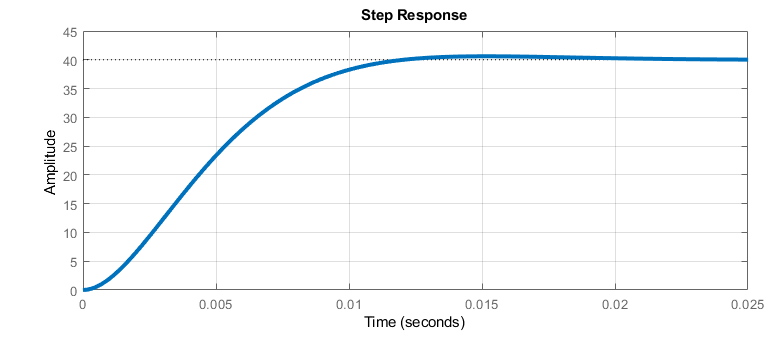
\includegraphics[width=12cm]{images/TD/step_BO.png}
\end{center}
	
	\item Identifiez le paramètre $G_0$.
	\answer{
		Par analyse graphique, on trouve que $V_{Sfinal} = 40\operatorname{V}$ lorsqu'on applique un échelon de tension unitaire ($V_E = 1\operatorname{V}$).
		
		On trouve alors $G_0 = 40$.
	}
	
	\item On obtient une valeur de $m = 0.8$ et de fréquence caractéristique $f_c = 55\operatorname{Hz}$. Est-ce cohérent avec la réponse obtenue ?
	\answer{
		$m = 0.8$ correspond à un système à la limite de la résonance. On remarque un léger dépassement autour de $15\operatorname{ms}$. Ce qui est cohérent.
		
		$f_c = 55\operatorname{Hz}$ donne un temps caractéristique d'environ $3\operatorname{ms}$. Là encore, c'est cohérent par rapport au temps de montée du système.
	}
	
	\item Tracez le diagramme de Bode de ce système.
	\answer{
		\begin{center}
			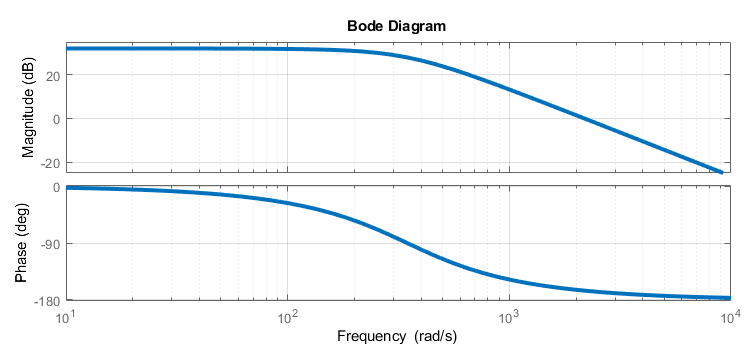
\includegraphics[width=14cm]{images/TD/bode_BO.png}
		\end{center}
	}
\end{enumerate}

%%%%%%%%%%%%%%%%%%%%%%%%%%%%%%%%%%%%%%%%%%%%%%%%%%%%%%%%%%%%%%%%%%
\encadreTDExo{2 - Système asservi non corrigé}{
\begin{itemize}[label=$\triangleright$,leftmargin=*]
	\item Caractérisation en fréquence d'un système asservi
\end{itemize}
}

On souhaite maintenant étudié le système asservi, sans correcteur pour l'instant ($C(p) = 1$).

\begin{enumerate}
	\item Quelle est la fonction de transfert en boucle fermée du système ?
	\answer{
		$$T_{BF}(p) = \frac{T(p)}{1 + T(p) \cdot K_{capt}}$$
		
		Après calcul, on obtient :
		
		$$T_{BF}(p) = \frac{G_0}{1 + G_0 \cdot K_{capt}} \cdot \frac{1}{1 + \frac{2 \cdot m \cdot p}{\omega_c \cdot (1 + G_0 \cdot K_{capt}} + \frac{p^2}{\omega_c^2 \cdot (1 + G_0 \cdot K_{capt}}}$$
	}
	
	\item Que valent les nouvelles caractéristiques de ce système (ordre, pulsation propre, amortissement...) ?
	\answer{
		Par identification dans la formule précédente :
		
		$$G_{0BF} = \frac{G_0}{1 + G_0 \cdot K_{capt}} = 0.0998$$
		
		$$f_{cBF} = f_c \cdot \sqrt{1 + G_0 \cdot K_{capt}} = 1100\operatorname{Hz} $$
		
		$$m_{BF} = \frac{m}{\sqrt{1 + G_0 \cdot K_{capt}}} = 0.04$$

	}
	
	\item Tracez son diagramme de Bode.
	\answer{
		\begin{center}
			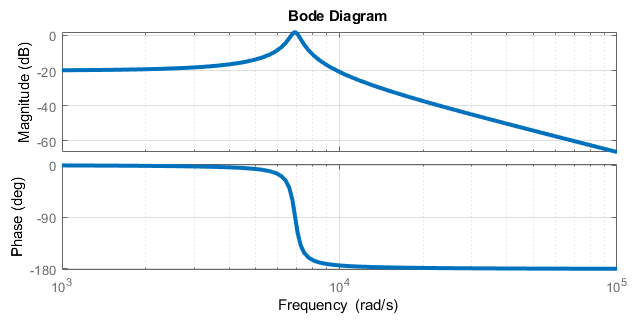
\includegraphics[width=14cm]{images/TD/bode_BF.png}
		\end{center}
	}
	
	\item La réponse à un échelon suivante est-elle celle de ce système ?
		\begin{center}
			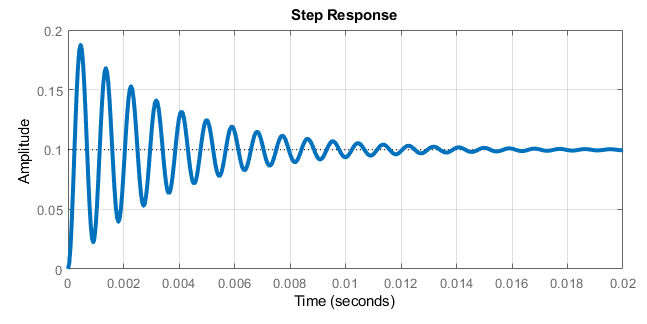
\includegraphics[width=14cm]{images/TD/step_BF.png}
		\end{center}	
	\answer{
		L'amplification statique (valeur finale du signal de sortie / valeur de l'échelon) est de 0.1, ce qui correspond au gain de $-20\operatorname{dB}$ dans la bande-passante.
	
		Il y a dépassement, représentant un amortissement faible. Cela est également cohérent avec la résonance apparente du diagramme de Bode.
		
		Enfin, la période des oscillations est de l'ordre de $1\operatorname{ms}$, ce qui équivaut à une fréquence de l'ordre de $1\operatorname{kHz}$. La fréquence de la résonance est autour de $7\operatorname{krd/s}$ (environ $1\operatorname{kHz}$). 
		
		Cette réponse indicielle peut correspondre à celle de ce système.
	}
	
\end{enumerate}

%%%%%%%%%%%%%%%%%%%%%%%%%%%%%%%%%%%%%%%%%%%%%%%%%%%%%%%%%%%%%%%%%%
\encadreTDExo{3 - Correcteur PID}{
\begin{itemize}[label=$\triangleright$,leftmargin=*]
	\item Caractérisation en fréquence d'un correcteur Proportionnel Intégral Dérivé
\end{itemize}
}

On souhaite corriger ce système avec un correcteur de type Proportionnel Intégral Dérivé (PID). Une forme, dite idéale, de ce correcteur est donné par la relation suivante :

$$C(p) = K \cdot (1 + \frac{1}{K_i \cdot p} + K_d \cdot p)$$

On ne s'intéressera pas ici au réglage de ce correcteur. Il existe pour cela différentes approches, dont celle de Ziegler-Nichols. Nous allons voir quel est l'intérêt des composantes proportionnelle et intégrale d'un correcteur.

\begin{enumerate}
	\item Mettez ce système sous forme d'un schéma bloc.
	\answer{
		\begin{center}
			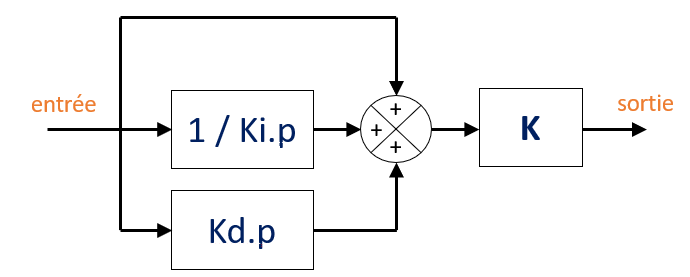
\includegraphics[width=10cm]{images/TD/correcteur_schema.png}
		\end{center}
	}
	
	\item Donnez la forme canonique de l'expression de $C(p)$.
	\answer{
		$$C(p) = \frac{K + K \cdot K_i \cdot p + K \cdot K_d \cdot K_i \cdot p^2}{K_i \cdot p}$$	
	}
	
	\item Quelles sont les unités des coefficients $K$, $K_i$ et $K_d$ ?
	\answer{
		$K$ est une amplification, sans unité.
		
		$K_i$ et $K_d$ sont des constantes de temps, en secondes.	
	}
	
	\medskip
	
	On commence par ajouter une composante $K$, les composantes intégrales et dérivées sont déconnectées.
	
	\item Que devient la fonction de transfert en boucle fermée du système asservi et corrigé ? Que deviennent les grandeurs caractéristiques de ce système ?
	\answer{
		$$T_{BF}(p) = \frac{K \cdot T(p)}{1 + K \cdot T(p) \cdot K_{capt}}$$
		
		Après calcul, on obtient :
		
		$$T_{BF}(p) = \frac{K \cdot G_0}{1 + K \cdot G_0 \cdot K_{capt}} \cdot \frac{1}{1 + \frac{2 \cdot m \cdot p}{\omega_c \cdot (1 + G_0 \cdot K\cdot K_{capt}} + \frac{p^2}{\omega_c^2 \cdot (1 + G_0 \cdot K \cdot K_{capt}}}$$	
		
		
		Par identification dans la formule précédente :
		
		$$G_{0BF} = \frac{K \cdot G_0}{1 + K \cdot G_0 \cdot K_{capt}}$$
		
		$$f_{cBF} = f_c \cdot \sqrt{1 + G_0 \cdot K \cdot K_{capt}}$$
		
		$$m_{BF} = \frac{m}{\sqrt{1 + G_0 \cdot K \cdot K_{capt}}}$$
	}
	
	\item Que valent ces valeurs pour $K = 10$ ? Pour $K = 0.1$ ?
	
	\answer{
		\textbf{Pour $K = 10$ :}
		
		$$G_{0BF} = \frac{K \cdot G_0}{1 + K \cdot G_0 \cdot K_{capt}} = 0.1$$
		
		$$f_{cBF} = f_c \cdot \sqrt{1 + G_0 \cdot K \cdot K_{capt}} = 3.48\operatorname{kHz}$$
		
		$$m_{BF} = \frac{m}{\sqrt{1 + G_0 \cdot K \cdot K_{capt}}} = 0.0126$$
		
		\textbf{Pour $K = 0.1$ :}
		
		$$G_{0BF} = \frac{K \cdot G_0}{1 + K \cdot G_0 \cdot K_{capt}} = 0.0976$$
		
		$$f_{cBF} = f_c \cdot \sqrt{1 + G_0 \cdot K \cdot K_{capt}} = 352\operatorname{kHz}$$
		
		$$m_{BF} = \frac{m}{\sqrt{1 + G_0 \cdot K \cdot K_{capt}}} = 0.125$$	
	}
	
	\item Tracez les diagrammes de Bode de ces deux systèmes sur le même diagramme que précédemment.
	\answer{
		\begin{center}
			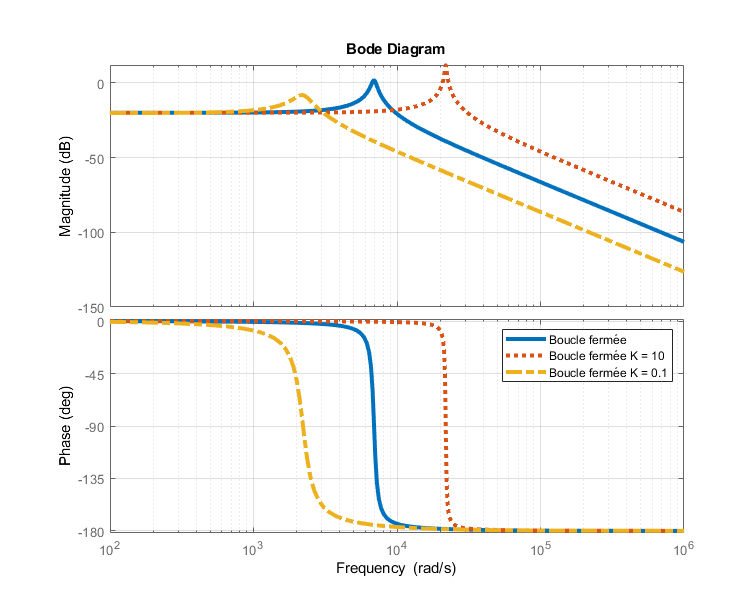
\includegraphics[width=14cm]{images/TD/bode_K_corr.png}
		\end{center}
	}
	\answer{
		On peut aussi s'intéresser aux réponses indicielles de ces 3 systèmes :
		\begin{center}
			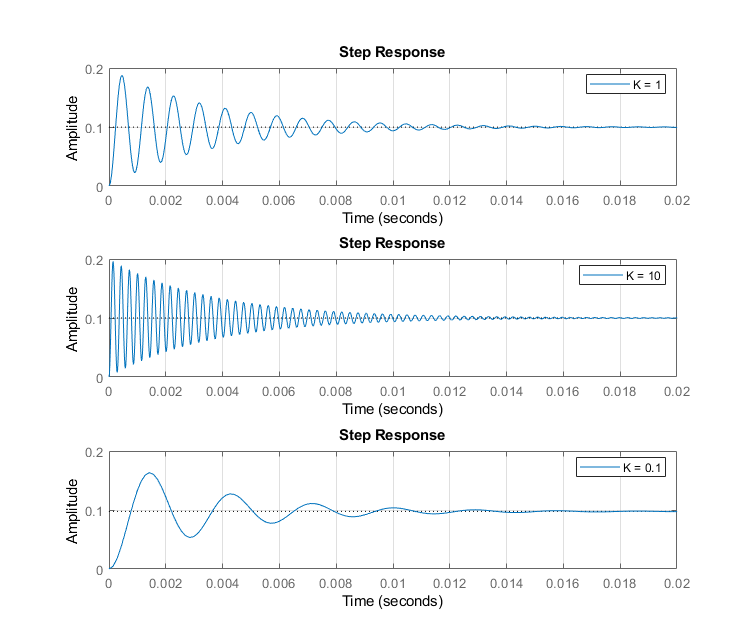
\includegraphics[width=14cm]{images/TD/step_K_corr.png}
		\end{center}
	}

	\medskip
	
	On ajoute la composante intégrale au correcteur.
	
	\item Que devient la fonction de transfert en boucle fermée du système asservi et corrigé ? 
	\answer{
		$$T_{BF}(p) = \frac{C(p) \cdot T(p)}{1 + K_{capt} \cdot C(p) \cdot T(p)}$$
		
		On posera $M = K_{capt} \cdot K \cdot G_0$.		
		
		Après calcul, on obtient :
		
		$$T_{BF}(p) = \frac{K \cdot G_0}{1 + M} \cdot \frac{1 + \tau_i \cdot p}{1 + \frac{p}{1 + M} \cdot (\frac{2 \cdot m}{\omega_c} + \tau_i \cdot M) + \frac{p^2}{\omega_c^2 \cdot (1 + M)}}$$
	}
	
	\medskip	
	
	Selon le choix des coefficients $K$ et $K_i$, le système peut être corrigé, mais peut également devenir instable...
	
	\begin{center}
		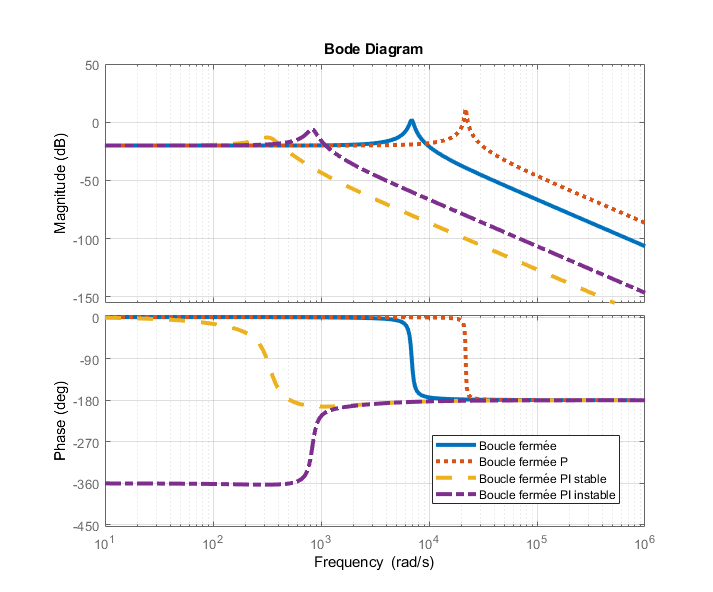
\includegraphics[width=14cm]{images/TD/bode_PI_corr.png}
	\end{center}	
	
	\begin{center}
		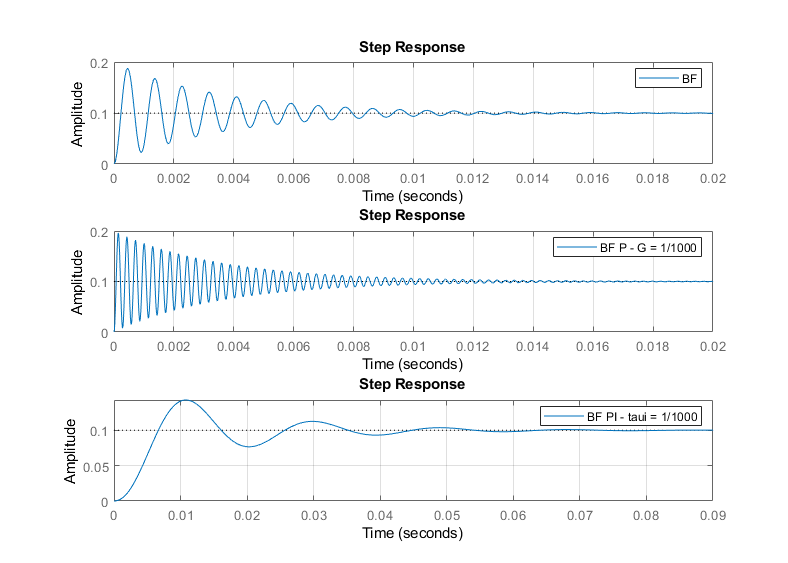
\includegraphics[width=14cm]{images/TD/step_PI_corr.png}
	\end{center}
	
\end{enumerate}